% !TeX encoding = UTF-8
% !TeX spellcheck = fr_FR
\documentclass[french,12pt,a4paper,titlepage,openright,openbib]{report}

\usepackage[utf8]{inputenc}
\usepackage[T1]{fontenc}
\usepackage[english,french]{babel}
\usepackage[default]{gillius}

\usepackage{graphicx}
\usepackage{lipsum}
\usepackage{array}
\usepackage[pdfborder={0 0 0}]{hyperref}
\usepackage[xindy,toc]{glossaries}
\usepackage{titlesec}
\usepackage{color}
\usepackage{blindtext}
\usepackage{fancyhdr}
\usepackage{lastpage}
\usepackage[pages=some]{background}
\usepackage[pass]{geometry}
\usepackage{afterpage}
\usepackage{emptypage}
\usepackage{fancybox}


% !TeX encoding = UTF-8
% !TeX spellcheck = fr_FR
% !TeX root = RapportMi3A.tex

%defini le style de couverture
\fancypagestyle{couverture}{
	\fancyhf{}
	\renewcommand \headrulewidth{0pt}
	\renewcommand \footrulewidth{0pt}
}

%default header & footer
\fancyhf{}
%redefinition du footer
\fancyfoot[C]{Page \textbf{\thepage} sur \textbf{\pageref{LastPage}}}
\renewcommand \footrulewidth{0pt}

%definition du header
\fancyhead[L]{\raisebox{-0.2 \height}{
\includegraphics[width=2cm]{logo_nxp}}}
\fancyhead[R]{\textsc Rapport de mi-parcours 3A}
\renewcommand \headrulewidth{0pt}

%colors
\definecolor{gray75}{gray}{0.75}
\definecolor{aqua}{RGB}{0,164,167}
\definecolor{petrol}{RGB}{0,112,136}

\definecolor{nxpblue}{RGB}{123,177,219}
\definecolor{nxporange}{RGB}{249,181,0}
\definecolor{nxpgreen}{RGB}{201,210,0}

\parindent=0in
\parskip=8pt

%margins 1 inch
\addtolength{\oddsidemargin}{-.5in}
\addtolength{\evensidemargin}{-.5in}
\addtolength{\textwidth}{1.2in}

\addtolength{\topmargin}{-.5in}
\addtolength{\textheight}{0.8in}

%ajoute une page blanche
\newcommand{\blankpage}{%
	\null
	\thispagestyle{empty}%
	\addtocounter{page}{-1}%
	\newpage}
%ajouter un hespace de 20pt
\newcommand{\hsp}{\hspace{20pt}}
%numérotaiton romaine
\renewcommand\thechapter{\Roman{chapter}}
\renewcommand\thesection{\Roman{section}}
\renewcommand \thesubsection {\thesection.\Roman{subsection}}

%modification du style de chapitre
\titleformat{\chapter}[hang]{\Huge\bfseries}{\thechapter\hsp\textcolor{gray75}{|}\hsp}{0pt}{\Huge\bfseries}
\titlespacing{\chapter}{0pt}{0pt}{12pt}

%Renomme Bibliogrphy en
%\renewcommand{\bibname}{Références}

%redefini le style plain qui est utilisé sur les premières pages de chapitre
\fancypagestyle{plain}{%
	\fancyhf{} % clear all header and footer fields
	\fancyfoot[C]{Page \textbf{\thepage} sur \textbf{\pageref{LastPage}}} % except the center
	\fancyhead[L]{\raisebox{-0.2 \height}{
\includegraphics[width=2cm]{logo_nxp}}}
	\fancyhead[R]{\textsc Rapport de mi-parcours 3A}
	\renewcommand \headrulewidth{0pt}
	\renewcommand{\footrulewidth}{0pt}}



\graphicspath{{template/}{img/}}

\title{Rapport de mi-parcours de troisième année}
\author{Jennifer Gr\"{a}nicher}
\date{12 Février 2018}

\pagestyle{fancy}


\makeglossaries
\newglossaryentry{mifare}
{
	name=MIFARE,
	description={Marque de NXP incluant une large gamme de circuits intégrés sans contact},
}
\newglossaryentry{desfire}
{
	name=DESFire,
	description={Marque de la famille MIFARE qui permet de créer des systèmes de cartes sécurisées grâce à l'alliance de la cryptographie et du sans contact},
}
\newglossaryentry{mooc}
{
	name=MOOC,
	description={Massive Open Online Course, formation ou cours en ligne},
	plural=MOOCs
}
\newacronym{nfc}{NFC}{Near Field Communication}
\newacronym{jee}{JEE}{Java Entreprise Edition}

\begin{document}
% !TeX encoding = UTF-8
% !TeX spellcheck = fr_FR
% !TeX root = RapportMi3A.tex

\backgroundsetup{
	scale=1,
	color=black,
	opacity=1.0,
	angle=0,
	contents={%
		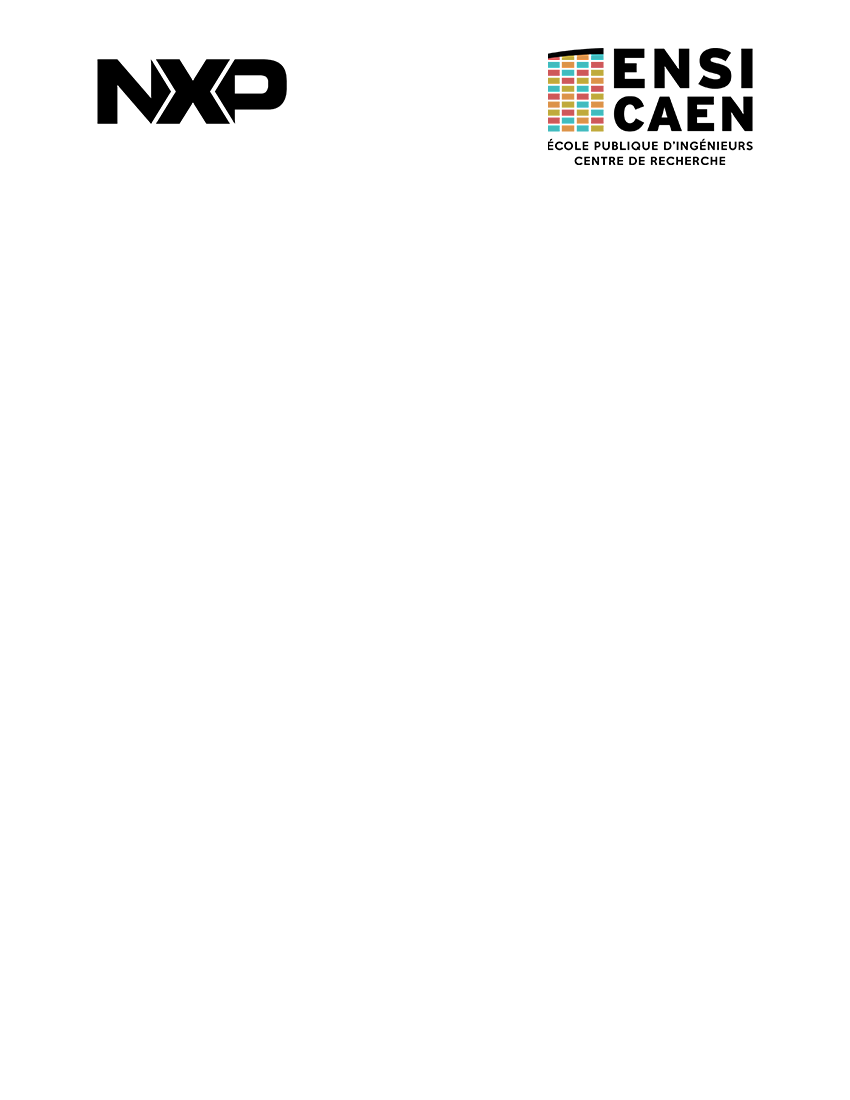
\includegraphics[width=\paperwidth, height=\paperheight]{cover_tmpl}
	}%
}

{
	\BgThispage
	\thispagestyle{couverture}
	
	\newgeometry{headheight=80pt, top=6cm, headsep=3cm}
	
	\makeatletter
	{\LARGE\bfseries\@title\par}
	{\color{aqua}Informatique par apprentissage \\
	\color{aqua}Année universitaire 2017-2018}
	\hfill
	\vspace{0.5cm}
	
	\includegraphics[width=15cm]{scylla}
	\vspace{0.5cm}
	
	\begin{minipage}[c]{0.5\textwidth}
	Tuteur école \par
	{\color{aqua} Wilfried \bsc{Aubry}}
	
	\vspace{0.5cm}
	
	Maître d'apprentissage \par
	{\color{aqua} Nicolas \bsc{Guillerm}}
	\end{minipage}
	\begin{minipage}[c]{0.5\textwidth}
	Tuteur école \par
	{\color{aqua} Wilfried \bsc{Aubry}}
	
	\vspace{0.5cm}
	
	Maître d'apprentissage \par
	{\color{aqua} Nicolas \bsc{Guillerm}}
	\end{minipage}
	
		
		
	
	\makeatother
	
	\vfill
	
	\afterpage{\blankpage}
	\restoregeometry
}


\maketitle

\chapter*{Remerciements}

J'aimerais remercier toutes les personnes qui ont contribué au bon déroulement de ces trois dernières années d'apprentissage, au sein de l'entreprise NXP Semiconductors, et au sein de l'ENSICAEN.

Je tiens particulièrement à remercier Virginie Jobard qui m'a épaulée et aidée à prendre mes repères au début.

Je souhaiterais également remercier Didier Graignic qui a su prendre le relais et m'aiguiller au cours de ma mission sur le projet MOOCTab.

J'aimerais aussi remercier Nicolas Guillerm pour toute l'aide qu'il a apporté que ce soit pour le rapport ou les missions au sein de l'entreprise.

Je remercie également Wilfried Aubry qui a été de bon conseil et qui a su apporter une grande aide.

Je tiens également à remercier mes collègues chez NXP pour leur aide et leurs soutien.


\tableofcontents

\chapter*{Historique}
\begin{table}[ht]
	\label{tab:historique}
	\centering
	\begin{tabular}{|c|c|c|c|}
		\hline
		{\bf Version} & {\bf Date} & {\bf Rédigé par}    & {\bf Mise à jour}    \\
		\hline
		1.0           & 29/01/2018 & Jennifer Gränicher  & Création du document \\
		\hline
		1.1           & 06/02/2018 & Jennifer Gränicher  & Mise en page \\
		\hline
	\end{tabular}
\end{table}

\vspace{2cm}

{\let \clearpage \relax \chapter*{Diffusion}}
\begin{table}[ht]
	\label{tab:diffusion}
	\centering
	\begin{tabular}{|c|c|c|c|}
		\hline
		{\bf Destinataire} & {\bf Société}      & {\bf Fonction}   		 & {\bf Date}\\
		\hline
		Nicolas Guillerm   & NXP Semiconductors & Maitre d'apprentissage & 08/02/2018 \\
		\hline
		Wifried Aubry      & ENSICAEN 			& Tuteur				 & 12/02/2018 \\
		\hline
	\end{tabular}
\end{table}

\chapter{Introduction}

Ce document parle de mes trois années d'apprentissage au sein de NXP Semiconductors, de Septembre 2015 à Janvier 2018.

Une première partie concerne les derniers changements au sein de l'entreprise.
Une seconde partie concerne les projets en cours, elle est centrée sur la dernière année.
Enfin, une autre partie traite de mon évolution personnelle et professionnelle au cours de ces trois années.

\chapter{Actualités}

Au cours des derniers mois les effectifs de NXP à Caen ont été réduits. Cela a eu pour conséquence un réaménagement de certains bureaux.
Didier Graignic qui remplaçait Virginie Jobard a quitté l'entreprise, lui aussi, Nicolas Guillerme l'a remplacé en qualité de maître d'apprentissage.
L'équipe avec laquelle je travaille est aujourd'hui composée de Nicolas Guillerme, Dominique Defossez et moi même. Cette équipe est l'équipe attachée au projet MOOCTab que je détaillerai plus loin.


\section{Qualcomm}

En octobre 2016 Qualcomm annonçait son souhait de racheter NXP Semiconductors. La commission américaine avait approuvé ce rachat mais la commisions européenne n'était pas d'accord. Après une enquête approfondie, la commission européenne accepte le rachat uniquement sous certaines conditions :
Qualcomm n'acquérira pas les brevets essentiels au standard \gls{nfc} de NXP, ni quelques uns non-essentiels concernant la \gls{nfc}.
Qualcomm devra maintenir, pendant une période de huit ans, la licence actuelle de la technologie \gls{mifare}. Enfin ils devront aussi garantir l'intéropérabilité des puces NXP avec les autres constructeurs.

\chapter{Missions}
Au cours de ma formation j'ai été amenée à travailler sur des petites tâches ponctuelles, principalement le développement d'application Android. Ces applications avaient pour but de montrer différents usages de la technologie \gls{nfc}.
En deuxième année mes tâches ont progressivement évoluée vers le projet européen MOOCTab qui occupe maintenant la plus grande partie de mon temps.
\section{MOOCTab}
MOOCTab est un projet européen qui réunit la Turquie et la France. Le but de ce projet est de proposer une solution permettant de consulter des \glspl{mooc} en ligne de manière sécurisée sur des tablettes. En outre la solution doit permettre de pouvoir passer des examens.

La solution comprend une MOOCBox qui permet aux utilisateurs de s'authentifier avec leurs badges et d'avoir accès au contenu qu'elle diffuse. NXP est chargé de réaliser la partie \gls{nfc} de cette box.
Le module \gls{nfc} de la box devra pouvoir lire les badges, potentiellement les écrire et partager des informations avec l'autre partie de la box.

Notre module est composé d'une petite carte tournant sous Android à laquelle nous avons rattachée une puce \gls{nfc} avec une antenne. Mon rôle a été de réaliser la liaison entre la carte avec la puce et l'antenne autant au niveau matériel que logiciel.

C'est pour moi une expérience inédite n'ayant jamais réalisé ce genre de tâches auparavant.
\section{NFC Playbook}
Il arrive que l'entreprise ait des besoins ponctuelles de produire des démonstrations ou des modèles pour promouvoir l'utilisation de la \gls{nfc} et notamment dans les applications mobiles.

Récemment un collègue d'un autre service est venu solliciter mes compétences en la matière afin de développer un petit squelette de code pouvant être réutilisé.
Le but était de produire une petite application Android permettant d'héberger des mini-applications qui utiliseraient la \gls{nfc}. Il fallait avoir la possibilité de lancer les mini-applications, soit en cliquant dessus, soit en utilisant un tag \gls{nfc}.

Cette application sera utilisée lors d'un évènement du Dôme qui aura lieu les 16 et 17 Février 2018 \cite{website:ledome}. C'est un atelier qui se fera sur une journée et sera centré sur le thème du livre et des intéractions numériques. Les développeurs et artistes de chaque équipe devront fabriquer des prototypes de livres améliorés grâce à l'outil numérique.

Cette mission m'a permis de faire une coupure par rapport au MOOCTab, tout en aidant un collègue. De plus ma contribution a permis d'éviter le recours à un prestataire et a donc induit des économies non négligeables.
\chapter{Évolution}
Lorsque je suis arrivée chez NXP la première fois je n'avais aucune expérience en entreprise. J'ai commencé par un stage de douze semaines, ce stage m'avait permis de faire mes premiers pas dans le monde professionnel et de trouver mon poste d'apprentie.
Cela fait maintenant deux ans et demi que j'évolue au fil des mois autant en entreprise qu'à l'école.
\section{Savoir-faire}
Les premières évolutions notables sont au niveau technique. J'ai abordé de nouvelles technologie, appris des langages que je ne connaissais pas, et assimilé de nouvelles compétences.
Lors de mon entrée en entreprise j'avais des connaissances dans quelques langages de programmation, avec une préférence pour les langages WEB, sans vraiment avoir pu approfondir la plupart d'entre eux.

J'ai été recrutée pour travailler sur des projets faisant l'emploi de la NFC, principalement du développement mobile sous Android, mais pas uniquement.

Mes premières missions on consisté à de la maintenance et du support sur des projets existants, Smartcampus et LabTab, cela m'a permis de progresser sur les langages \gls{jee} et Java pour Android. J'ai aussi pu appliquer des compétences en base de données ainsi qu'en installation et gestion de serveur.

Avec le temps, mes tâches ont évolué, on m'a confié de nouveaux projets à réaliser de A à Z.
Mon premier projet était un service de report d'incidents. Des tags NFC permettaient de simplifier le remplissage d'informations concernant l'endroit où se situait l'incident.
Bien que le développement Android fut indispensable pour la partie mobile, j'avais le choix pour les technologies utilisées pour le reste. J'ai alors décidé de me former sur une technologie que je ne connaissais pas: Spring, ceci tout en continuant d'appliquer ce que j'avais déjà acquis.

Finalement c'est sur le projet MOOCTab, qui a occupé la majeure partie de mon temps, que j'ai gagné le plus en compétences. J'ai du réaliser plusieurs démonstrateurs sous Android avec des bracelets connectés notamment. Jusqu'alors je n'avais travaillé que sur de simple tags NFC. Les bracelets remplaçaient l'utilisation de cartes pour s'identifier ou s'authentifier. J'ai découvert de toutes nouvelles technologies et concepts qui ne ressemblaient à rien de ce que j'avais pu faire jusque là.
Dans cet ensemble de nouveautés on peut citer : \gls{mifare} \gls{desfire} pour la création de cartes ainsi que la compilation de sources Android. C'est sans doute ce projet qui a été pour moi la clé d'une forte évolution technique.
\section{Savoir-être}
Ces projets ne m'ont pas uniquement permis de gagner en technicité mais aussi sur d'autres compétences.
Malgré le fait que je n'avais pas de problèmes à travailler en autonomie, j'avais besoin de beaucoup d'appui lors de mes débuts. Je manquais beaucoup de confiance en moi et en ce que j'étais capable de faire. Petit à petit et avec l'aide de mes maîtres d'apprentissage j'ai su surmonter mes difficultés.
Et au fil des projets, sans m'en rendre compte j'ai pris confiance en moi, ce qui a résulté en plus de prises d'initatives et en propositions de solutions.
Le travail en autonomie et la réalisation de divers projets m'a aussi permis d'améliorer ma gestion du temps et du stress.
\subsection{Collaboration}
J'ai beaucoup travaillé en autonomie sur les diverses missions qui m'ont été attribuées, je n'ai pu expérimenter le travail en équipe qu'au travers des projets de l'ENSICAEN. En revanche j'ai appris à solliciter d'autres professionnels lorsque cela était nécessaire. Lors du projet MOOCTab par exemple lorsque j'avais des difficultés techniques j'ai démandé des informations à d'autres collègues, j'ai aussi du requérir de l'aide sur des tâches qui n'étaient pas de mon ressort, du soudage de composants par exemple. Toujours au cours de cette mission, j'ai eu l'occasion de travailler en Collaboration avec d'autres entreprises, il était important d'échanger des informations afin d'intégrer le travail de chaqun pour obtenir un produit final cohérent.
\chapter{Bilan}
\lipsum[6-7]
\chapter{Conclusion}
\lipsum[8-9]

\printglossary[title={Glossaire}]

\bibliography{mybib}
\bibliographystyle{plain}
	
\end{document}


